Konstruieren Sie zu jeder der folgenden Sprachen einen
endlichen Automaten, der genau diese Sprache akzeptiert.
Die Sprachen verwenden die Alphabete
$\Sigma_1=\{{\tt a},{\tt b}\}$ und
$\Sigma_2=\{{\tt 0},{\tt 1}\}$.
\begin{teilaufgaben}
\item
$L=\{w\in \Sigma_1^*|\text{
$w$ beginnt mit \texttt{a} und enthält höchstens ein \texttt{b}
}\}$
\item
$L=\{w\in \Sigma_1^*|\text{
$w$ enthält eine gerade Anzahl {\tt a}s und mindestens
zwei {\tt b}s
}\}$
\item
$L=\{w\in \Sigma_1^*|\text{
$w$ hat gerade Länge und eine ungerade Anzahl {\tt b}s
}\}$
\item
$L=\{w\in \Sigma_1^*|\text{
$w$ enthält nicht genau zwei {\tt a}s
}\}$
\item
$L=\{w\in \Sigma_2^*|\text{
an jeder ungeraden Position von $w$ steht ein {\tt 1}
}\}$
\item
$L=\{w\in \Sigma_2^*|\;|w|\le 5\}$
\item
$L=\emptyset\subset \Sigma_2^*$
\end{teilaufgaben}

\thema{DEA}
\thema{Zustandsdiagramm}

\begin{loesung}
\begin{teilaufgaben}
%
% a)
%
\item
Die Zustände haben folgende Bedeutung:
\begin{center}
\begin{tabular}{c|l}
Zustand&Bedeutung\\
\hline
$z_0$&Startzeichen des Wortes noch nicht verarbeitet
\\
$z_1$&beginnt mit {\tt a}, noch kein {\tt b}
\\
$z_2$&beginnt mit {\tt a}, genau ein {\tt b}
\\
$z_3$&beginnt mit {\tt b} oder mehr als ein {\tt b}
\\
\end{tabular}
\end{center}
%\[
%\entrymodifiers={++[o][F]}
%\xymatrix @-1mm {
%*+\txt{} \ar[r]
%        &{z_0} \ar[r]^{\tt a} \ar[d]^{\tt b}
%                &*++[o][F=]{z_1} \ar[d]^{\tt b} \ar@(dr,ur)_{\tt a}
%\\
%*+\txt{}
%        &{z_3} \ar@(dr,dl)^{{\tt a},{\tt b}}
%                &*++[o][F=]{z_2} \ar@(dr,dl)^{\tt a} \ar[l]^{\tt b}
%}
%\]
\begin{center}
\begin{tikzpicture}[>=latex,thick]
\def\l{1.6}
\coordinate (z0) at (0,0);
\coordinate (z1) at ({\l},0);
\coordinate (z2) at ({\l},{-\l});
\coordinate (z3) at (0,{-\l});
\node at (z0) {$z_0$};
\node at (z1) {$z_1$};
\node at (z2) {$z_2$};
\node at (z3) {$z_3$};
\draw (z0) circle[radius=0.35];
\draw (z1) circle[radius=0.35];
\draw (z1) circle[radius=0.30];
\draw (z2) circle[radius=0.35];
\draw (z2) circle[radius=0.30];
\draw (z3) circle[radius=0.35];
\draw[->,shorten <= 0.35cm,shorten >= 0.35cm] ({-\l},0) -- (z0);
\draw[->,shorten <= 0.35cm,shorten >= 0.35cm] (z0) -- (z1);
\draw[->,shorten <= 0.35cm,shorten >= 0.35cm] (z0) -- (z3);
\draw[->,shorten <= 0.35cm,shorten >= 0.35cm] (z1) -- (z2);
\draw[->,shorten <= 0.35cm,shorten >= 0.35cm] (z2) -- (z3);
\draw[->,shorten <= 0.35cm,shorten >= 0.35cm]
	(z1) to[out=-30,in=30,distance=1.2cm] (z1);
\draw[->,shorten <= 0.35cm,shorten >= 0.35cm]
	(z2) to[out=-60,in=-120,distance=1.2cm] (z2);
\draw[->,shorten <= 0.35cm,shorten >= 0.35cm]
	(z3) to[out=-60,in=-120,distance=1.2cm] (z3);
\node at ($0.5*(z0)+0.5*(z1)+(0,-0.1)$) [above] {\texttt{a}\strut};
\node at ($0.5*(z2)+0.5*(z3)+(0,0.1)$) [below] {\texttt{b}\strut};
\node at ($0.5*(z0)+0.5*(z3)$) [left] {\texttt{b}\strut};
\node at ($0.5*(z1)+0.5*(z2)$) [right] {\texttt{b}\strut};
\node at ($(z3)+(0,-1.1)$) {\texttt{a},\texttt{b}\strut};
\node at ($(z2)+(0,-1.1)$) {\texttt{a}\strut};
\node at ($(z1)+(1.1,0)$) {\texttt{a}\strut};
\end{tikzpicture}
\end{center}

Selbstverständlich kann man diese Aufgabe auch mit Hilfe des Satzes~3.4
aus der Vorlesung lösen. Dazu müssen die Mengen $L(w)$ bestimmt
werden:
\begin{center}
\begin{tabular}{|c|l|c|}
\hline
$w$&$L(w)$&$z_{?}$\\
\hline
$\varepsilon$&$L$&$z_0$\\
\tt a&$\{w'\in\Sigma_1^*\,|\,\text{$w'$ enthält höchstens ein {\tt b}}\}$&$z_1$\\
\tt b&$\emptyset$&$z_3$\\
\tt aa&$\{w'\in\Sigma_1^*\,|\,\text{$w'$ enthält höchstens ein {\tt b}}\}$&$z_1$\\
\tt ab&$\{w'\in\Sigma_1^*\,|\,|w'|_{\tt b} = 0\}$&$z_2$\\
\tt ba&$\emptyset$&$z_3$\\
\tt bb&$\emptyset$&$z_3$\\
$\vdots$&$\vdots$&\\
\hline
\end{tabular}
\end{center}
Offenbar gibt es vier verschiedene Mengen, also kommt der DEA von $L$
mit 4 Zuständen aus. $L(\texttt{a})$ und $L(\texttt{ab})$ enthälten das
leere Wort, sind als Akzeptierzustände. Die "Ubergänge können ebenfalls
aus der Tabelle abgelesen werden, es ergibt sich der gleiche Automat.

%
% b)
%
\item Die Zeilen zählen die Anzahl \texttt{b}, die bereits gelesen
wurden, die Spalten führen Buch über den Zweierrest der Anzahl
\texttt{a}.
%\[
%\entrymodifiers={++[o][F]}
%\xymatrix @-1mm {
%*+\txt{} \ar[r]
%        &{z_0}\ar@/^/[r]^{\tt a} \ar[d]^{\tt b}
%                &{z_1}\ar@/^/[l]^{\tt a} \ar[d]^{\tt b}
%\\
%*+\txt{}
%        &{z_2}\ar@/^/[r]^{\tt a} \ar[d]^{\tt b}
%                &{z_3}\ar@/^/[l]^{\tt a} \ar[d]^{\tt b}
%\\
%*+\txt{}
%        &*++[o][F=]{z_4}\ar@/^/[r]^{\tt a} \ar@(dr,dl)^{\tt b}
%                &{z_5}\ar@/^/[l]^{\tt a} \ar@(dr,dl)^{\tt b}
%}
%\]
\begin{center}
\begin{tikzpicture}[>=latex,thick]
\def\l{1.6}
\coordinate (z0) at (0,0);
\coordinate (z1) at (\l,0);
\coordinate (z2) at (0,{-\l});
\coordinate (z3) at (\l,{-\l});
\coordinate (z4) at (0,{-2*\l});
\coordinate (z5) at (\l,{-2*\l});
\node at (z0) {$z_0$};
\node at (z1) {$z_1$};
\node at (z2) {$z_2$};
\node at (z3) {$z_3$};
\node at (z4) {$z_4$};
\node at (z5) {$z_5$};
\draw (z0) circle[radius=0.35];
\draw (z1) circle[radius=0.35];
\draw (z2) circle[radius=0.35];
\draw (z3) circle[radius=0.35];
\draw (z4) circle[radius=0.35];
\draw (z4) circle[radius=0.30];
\draw (z5) circle[radius=0.35];
\draw[->,shorten <= 0.35cm,shorten >= 0.35cm] (-\l,0) -- (z0);
\draw[->,shorten <= 0.35cm,shorten >= 0.35cm] (z0) -- (z2);
\draw[->,shorten <= 0.35cm,shorten >= 0.35cm] (z1) -- (z3);
\draw[->,shorten <= 0.35cm,shorten >= 0.35cm] (z2) -- (z4);
\draw[->,shorten <= 0.35cm,shorten >= 0.35cm] (z3) -- (z5);
\draw[->,shorten <= 0.35cm,shorten >= 0.35cm]
	(z0) to[out=20,in=160] (z1);
\draw[->,shorten <= 0.35cm,shorten >= 0.35cm]
	(z1) to[out=-160,in=-20] (z0);
\draw[->,shorten <= 0.35cm,shorten >= 0.35cm]
	(z2) to[out=20,in=160] (z3);
\draw[->,shorten <= 0.35cm,shorten >= 0.35cm]
	(z3) to[out=-160,in=-20] (z2);
\draw[->,shorten <= 0.35cm,shorten >= 0.35cm]
	(z4) to[out=20,in=160] (z5);
\draw[->,shorten <= 0.35cm,shorten >= 0.35cm]
	(z5) to[out=-160,in=-20] (z4);
\draw[->,shorten <= 0.35cm,shorten >= 0.35cm]
	(z5) to[out=-60,in=-120,distance=1.2cm] (z5);
\draw[->,shorten <= 0.35cm,shorten >= 0.35cm]
	(z4) to[out=-60,in=-120,distance=1.2cm] (z4);
\node at ($(z4)+(0,-1.1)$) {\texttt{b}};
\node at ($(z5)+(0,-1.1)$) {\texttt{b}};
\node at ($0.5*(z0)+0.5*(z1)+(0,0.4)$) {\texttt{a}};
\node at ($0.5*(z0)+0.5*(z1)+(0,-0.4)$) {\texttt{a}};
\node at ($0.5*(z2)+0.5*(z3)+(0,0.4)$) {\texttt{a}};
\node at ($0.5*(z2)+0.5*(z3)+(0,-0.4)$) {\texttt{a}};
\node at ($0.5*(z4)+0.5*(z5)+(0,0.4)$) {\texttt{a}};
\node at ($0.5*(z4)+0.5*(z5)+(0,-0.4)$) {\texttt{a}};
\node at ($0.5*(z0)+0.5*(z2)$) [left] {\texttt{b}};
\node at ($0.5*(z2)+0.5*(z4)$) [left] {\texttt{b}};
\node at ($0.5*(z1)+0.5*(z3)$) [right] {\texttt{b}};
\node at ($0.5*(z3)+0.5*(z5)$) [right] {\texttt{b}};
\end{tikzpicture}
\end{center}
Lösung mit Myhill-Nerode: Startzustand ist $L$, weitere Mengen
der Form $L(w)$ sind
\begin{center}
\begin{tabular}{c|ll|c}
$w$&$L(w)$&$z_i$&$\varepsilon\in L(w)$\\
\hline
$\varepsilon$&$L$&$=L_0$&nein\\
  {\tt a}&$\{w'\in\Sigma_1^*\;|\;\text{$|w'|_{\text{\tt a}}$ ungerade, $|w'|_{\text{\tt b}}\ge 2$}\}$&$=L_1$&nein\\
  {\tt b}&$\{w'\in\Sigma_1^*\;|\;\text{$|w'|_{\text{\tt a}}$ gerade,   $|w'|_{\text{\tt b}}\ge 1$}\}$&$=L_2$&nein\\
 {\tt aa}&$\{w'\in\Sigma_1^*\;|\;\text{$|w'|_{\text{\tt a}}$ gerade,   $|w'|_{\text{\tt b}}\ge 2$}\}$&$=L_0$&nein\\
 {\tt ab}&$\{w'\in\Sigma_1^*\;|\;\text{$|w'|_{\text{\tt a}}$ ungerade, $|w'|_{\text{\tt b}}\ge 1$}\}$&$=L_3$&nein\\
 {\tt bb}&$\{w'\in\Sigma_1^*\;|\;\text{$|w'|_{\text{\tt a}}$ gerade,   $|w'|_{\text{\tt b}}\ge 0$}\}$&$=L_4$&ja\\
{\tt aaa}&$\{w'\in\Sigma_1^*\;|\;\text{$|w'|_{\text{\tt a}}$ ungerade, $|w'|_{\text{\tt b}}\ge 2$}\}$&$=L_1$&nein\\
{\tt aab}&$\{w'\in\Sigma_1^*\;|\;\text{$|w'|_{\text{\tt a}}$ gerade,   $|w'|_{\text{\tt b}}\ge 1$}\}$&$=L_2$&nein\\
{\tt abb}&$\{w'\in\Sigma_1^*\;|\;\text{$|w'|_{\text{\tt a}}$ ungerade, $|w'|_{\text{\tt b}}\ge 0$}\}$&$=L_5$&nein\\
{\tt bbb}&$\{w'\in\Sigma_1^*\;|\;\text{$|w'|_{\text{\tt a}}$ gerade,   $|w'|_{\text{\tt b}}\ge 0$}\}$&$=L_4$&ja\\
\hline
\end{tabular}
\end{center}
Die Zustände $L_i$ entsprechen den $z_i$ im Zustandsdiagramm.

%
% c)
%
\item Die Zeilen codieren den Zweierrest der Anzahl {\tt b}s,
die Spalten den Zweierrest der Länge von $w$.
%\[
%\entrymodifiers={++[o][F]}
%\xymatrix @-1mm {
%*+\txt{} \ar[r]
%        &{z_0} \ar@/^/[r]^{\tt a} \ar@/^/[dr]_{\tt b}
%                &{z_1} \ar@/^/[l]_{\tt a}\ar@/^/[dl]%^{\tt b}
%\\
%*+\txt{}
%        &*++[o][F=]{z_2}\ar@/^/[r]_{\tt a}\ar@/^/[ur]
%                &{z_3} \ar@/^/[l]^{\tt a}\ar@/^/[ul]
%}
%\]
\begin{center}
\begin{tikzpicture}[>=latex,thick]
\def\l{1.8}
\coordinate (z0) at (0,0);
\coordinate (z1) at (\l,0);
\coordinate (z2) at (0,{-\l});
\coordinate (z3) at (\l,{-\l});
\node at (z0) {$z_0$};
\node at (z1) {$z_1$};
\node at (z2) {$z_2$};
\node at (z3) {$z_3$};
\draw (z0) circle[radius=0.35];
\draw (z1) circle[radius=0.35];
\draw (z2) circle[radius=0.35];
\draw (z2) circle[radius=0.30];
\draw (z3) circle[radius=0.35];
\draw[->,shorten <= 0.35cm,shorten >= 0.35cm] ($(z0)+(-\l,0)$) -- (z0);
\draw[->,shorten <= 0.35cm,shorten >= 0.35cm] (z0) to[out=20,in=160] (z1);
\draw[->,shorten <= 0.35cm,shorten >= 0.35cm] (z2) to[out=20,in=160] (z3);
\draw[->,shorten <= 0.35cm,shorten >= 0.35cm] (z1) to[out=-160,in=-20] (z0);
\draw[->,shorten <= 0.35cm,shorten >= 0.35cm] (z3) to[out=-160,in=-20] (z2);
\draw[->,shorten <= 0.35cm,shorten >= 0.35cm] (z0) to[out=-30,in=120] (z3);
\draw[->,shorten <= 0.35cm,shorten >= 0.35cm] (z2) to[out=30,in=-120] (z1);
\draw[->,shorten <= 0.35cm,shorten >= 0.35cm] (z3) to[out=150,in=-60] (z0);
\draw[->,shorten <= 0.35cm,shorten >= 0.35cm] (z1) to[out=-150,in=60] (z2);
\node at ($0.25*(z0)+0.25*(z1)+0.25*(z2)+0.25*(z3)$) {\texttt{b}};
\node at ($0.5*(z0)+0.5*(z1)$) {\texttt{a}};
\node at ($0.5*(z2)+0.5*(z3)$) {\texttt{a}};
\end{tikzpicture}
\end{center}
Lösung mit Myhill-Nerode: Als Zustände findet man die folgenden
Mengen:
\begin{center}
\begin{tabular}{c|ll|c}
$w$&$L(w)$&$z_i$&$\varepsilon\in L(w)$\\
\hline
$\varepsilon$&$L$&$=L_0$&nein\\
  {\tt a}&$\{w'\in\Sigma_1^*\;|\;\text{$|w'|$ ungerade, $|w'|_{\text{\tt b}}$ ungerade}\}$&$=L_1$&nein\\
  {\tt b}&$\{w'\in\Sigma_1^*\;|\;\text{$|w'|$ ungerade, $|w'|_{\text{\tt b}}$   gerade}\}$&$=L_3$&nein\\
 {\tt aa}&$\{w'\in\Sigma_1^*\;|\;\text{$|w'|$ gerade,   $|w'|_{\text{\tt b}}$ ungerade}\}$&$=L_0$&nein\\
 {\tt ab}&$\{w'\in\Sigma_1^*\;|\;\text{$|w'|$ gerade,   $|w'|_{\text{\tt b}}$   gerade}\}$&$=L_2$&ja\\
 {\tt bb}&$\{w'\in\Sigma_1^*\;|\;\text{$|w'|$ gerade,   $|w'|_{\text{\tt b}}$ ungerade}\}$&$=L_0$&nein\\
{\tt aaa}&$\{w'\in\Sigma_1^*\;|\;\text{$|w'|$ ungerade, $|w'|_{\text{\tt b}}$ ungerade}\}$&$=L_1$&nein\\
{\tt aab}&$\{w'\in\Sigma_1^*\;|\;\text{$|w'|$ ungerade, $|w'|_{\text{\tt b}}$   gerade}\}$&$=L_3$&nein\\
{\tt abb}&$\{w'\in\Sigma_1^*\;|\;\text{$|w'|$ ungerade, $|w'|_{\text{\tt b}}$ ungerade}\}$&$=L_1$&nein\\
{\tt bbb}&$\{w'\in\Sigma_1^*\;|\;\text{$|w'|$ ungerade, $|w'|_{\text{\tt b}}$   gerade}\}$&$=L_3$&nein\\
\hline
\end{tabular}
\end{center}
Die Zustande $L_i$ entsprechen wieder den $z_i$ von vorhin.

\item
In den Zuständen $z_i,i <3$ hat das Worte genau $i$ {\tt a}s,
im Zustand $z_3$ hat das Wort 3 oder mehr {\tt a}s.
%\[
%\entrymodifiers={++[o][F]}
%\xymatrix @-1mm {
%*+\txt{} \ar[r]
%        &*++[o][F=]{z_0}\ar[r]^{\tt a} \ar@(dr,dl)^{\tt b}
%                &*++[o][F=]{z_1}\ar[r]^{\tt a} \ar@(dr,dl)^{\tt b}
%                        &{z_2} \ar@(dr,dl)^{\tt b} \ar[r]^{\tt a}
%                                &*++[o][F=]{z_3} \ar@(dr,dl)^{{\tt a},{\tt b}}
%}
%\]
\begin{center}
\begin{tikzpicture}[>=latex,thick]
\def\l{1.6}
\coordinate (z0) at (0,0);
\coordinate (z1) at (\l,0);
\coordinate (z2) at ({2*\l},0);
\coordinate (z3) at ({3*\l},0);
\node at (z0) {$z_0$};
\node at (z1) {$z_1$};
\node at (z2) {$z_2$};
\node at (z3) {$z_3$};
\draw (z0) circle[radius=0.35];
\draw (z0) circle[radius=0.30];
\draw (z1) circle[radius=0.35];
\draw (z1) circle[radius=0.30];
\draw (z2) circle[radius=0.35];
\draw (z3) circle[radius=0.35];
\draw (z3) circle[radius=0.30];
\draw[->,shorten <= 0.35cm,shorten >= 0.35cm] (-\l,0) -- (z0);
\draw[->,shorten <= 0.35cm,shorten >= 0.35cm] (z0) -- (z1);
\draw[->,shorten <= 0.35cm,shorten >= 0.35cm] (z1) -- (z2);
\draw[->,shorten <= 0.35cm,shorten >= 0.35cm] (z2) -- (z3);
\draw[->,shorten <= 0.35cm,shorten >= 0.35cm]
	(z0) to[out=-60,in=-120,distance=1.2cm] (z0);
\draw[->,shorten <= 0.35cm,shorten >= 0.35cm]
	(z1) to[out=-60,in=-120,distance=1.2cm] (z1);
\draw[->,shorten <= 0.35cm,shorten >= 0.35cm]
	(z2) to[out=-60,in=-120,distance=1.2cm] (z2);
\draw[->,shorten <= 0.35cm,shorten >= 0.35cm]
	(z3) to[out=-60,in=-120,distance=1.2cm] (z3);
\node at ($0.5*(z0)+0.5*(z1)$) [above] {\texttt{a}};
\node at ($0.5*(z1)+0.5*(z2)$) [above] {\texttt{a}};
\node at ($0.5*(z2)+0.5*(z3)$) [above] {\texttt{a}};
\node at ($(z0)+(0,-1.15)$) {\texttt{b}\strut};
\node at ($(z1)+(0,-1.15)$) {\texttt{b}\strut};
\node at ($(z2)+(0,-1.15)$) {\texttt{b}\strut};
\node at ($(z3)+(0,-1.15)$) {\texttt{a},\texttt{b}\strut};
\end{tikzpicture}
\end{center}
Lösung mit Myhill-Nerode:
\begin{center}
\begin{tabular}{c|ll|c}
$w$&$L(w)$&$z_i$&$\varepsilon\in L(w)$\\
\hline
$\varepsilon$&$L$&$=L_0$&ja\\
  {\tt a}&$\{w'\in\Sigma_1^*\;|\;\text{$|w'|_{\tt a}\ne 1$}\}$&$=L_1$&ja\\
  {\tt b}&$\{w'\in\Sigma_1^*\;|\;\text{$|w'|_{\tt a}\ne 2$}\}$&$=L_0$&ja\\
 {\tt aa}&$\{w'\in\Sigma_1^*\;|\;\text{$|w'|_{\tt a}\ne 0$}\}$&$=L_2$&nein\\
 {\tt ab}&$\{w'\in\Sigma_1^*\;|\;\text{$|w'|_{\tt a}\ne 1$}\}$&$=L_1$&ja\\
 {\tt ba}&$\{w'\in\Sigma_1^*\;|\;\text{$|w'|_{\tt a}\ne 1$}\}$&$=L_1$&ja\\
 {\tt bb}&$\{w'\in\Sigma_1^*\;|\;\text{$|w'|_{\tt a}\ne 2$}\}$&$=L_0$&ja\\
{\tt aaa}&$\Sigma_1^*$                                      &$=L_3$&ja\\
{\tt aab}&$\{w'\in\Sigma_1^*\;|\;\text{$|w'|_{\tt a}\ne 0$}\}$&$=L_2$&nein\\
{\tt aba}&$\{w'\in\Sigma_1^*\;|\;\text{$|w'|_{\tt a}\ne 0$}\}$&$=L_2$&nein\\
{\tt abb}&$\{w'\in\Sigma_1^*\;|\;\text{$|w'|_{\tt a}\ne 1$}\}$&$=L_1$&ja\\
{\tt baa}&$\{w'\in\Sigma_1^*\;|\;\text{$|w'|_{\tt a}\ne 0$}\}$&$=L_2$&nein\\
{\tt bab}&$\{w'\in\Sigma_1^*\;|\;\text{$|w'|_{\tt a}\ne 1$}\}$&$=L_1$&ja\\
{\tt bba}&$\{w'\in\Sigma_1^*\;|\;\text{$|w'|_{\tt a}\ne 1$}\}$&$=L_1$&ja\\
{\tt bbb}&$\{w'\in\Sigma_1^*\;|\;\text{$|w'|_{\tt a}\ne 2$}\}$&$=L_0$&ja\\
\hline
\end{tabular}
\end{center}

\item Bedeutung der Zustände:
\begin{center}
\begin{tabular}{c|l}
Zustand&Beschreibung\\
\hline
$z_0$&gerades Zeichen, Bedingung an ungeraden Stellen immer erfüllt\\
$z_1$&ungerades Zeichen war eine {\tt 1}\\
$z_2$&{\tt 0} an ungerader Stelle\\
\end{tabular}
\end{center}
%\[
%\entrymodifiers={++[o][F]}
%\xymatrix @-1mm {
%*+\txt{} \ar[r]
%        &*++[o][F=]{z_0}\ar@/^/[r]^{{\tt 1}} \ar[d]^{\tt 0}
%                &*++[o][F=]{z_1} \ar@/^/[l]^{{\tt 0},{\tt 1}}
%\\
%*+\txt{}
%        &{z_2}\ar@(ur,dr)^{{\tt 0},{\tt 1}}
%                &*+\txt{}
%}
%\]
\begin{center}
\begin{tikzpicture}[>=latex,thick]
\def\l{1.6}
\coordinate (z0) at (0,0);
\coordinate (z1) at (\l,0);
\coordinate (z2) at (0,-\l);
\draw (z0) circle[radius=0.35];
\draw (z0) circle[radius=0.30];
\draw (z1) circle[radius=0.35];
\draw (z1) circle[radius=0.30];
\draw (z2) circle[radius=0.35];
\node at (z0) {$z_0$};
\node at (z1) {$z_1$};
\node at (z2) {$z_2$};
\draw[->,shorten <= 0.35cm,shorten >= 0.35cm] (-\l,0) -- (z0);
\draw[->,shorten <= 0.35cm,shorten >= 0.35cm] (z0) -- (z2);
\draw[->,shorten <= 0.35cm,shorten >= 0.35cm] (z0) to[out=20,in=160] (z1);
\draw[->,shorten <= 0.35cm,shorten >= 0.35cm] (z1) to[out=-160,in=-20] (z0);
\draw[->,shorten <= 0.35cm,shorten >= 0.35cm] (z2) to[out=30,in=-30,distance=1.2cm] (z2);
\node at ($0.5*(z0)+0.5*(z1)+(0,0.4)$) {\texttt{1}\strut};
\node at ($0.5*(z0)+0.5*(z1)+(0,-0.4)$) {\texttt{0},\texttt{1}\strut};
\node at ($0.5*(z0)+0.5*(z2)$) [left] {\texttt{0}\strut};
\node at ($(z2)+(1.2,0)$) {\texttt{0},\texttt{1}\strut};
\end{tikzpicture}
\end{center}
Lösung mit Myhill-Nerode: Die Zustände sind
\begin{center}
\begin{tabular}{c|ll|c}
$w$&$L(w)$&$z_i$&$\varepsilon\in L(w)$\\
\hline
$\varepsilon$&$L$&$=L_0$&ja\\
  {\tt 0}&$\emptyset$&$=L_2$&ja\\
  {\tt 1}&$\{ w'\in\Sigma_2^*\;|\; \text{an jeder geraden Stelle eine {\tt 1}}\}$&$=L_1$&ja\\
 {\tt 00}&$\emptyset$&$=L_2$&nein\\
 {\tt 01}&$\emptyset$&$=L_2$&nein\\
 {\tt 10}&$L$&$=L_0$&ja\\
 {\tt 11}&$L$&$=L_0$&ja\\
{\tt 000}&$\emptyset$&$=L_2$&nein\\
{\tt 001}&$\emptyset$&$=L_2$&nein\\
{\tt 010}&$\emptyset$&$=L_2$&nein\\
{\tt 011}&$\emptyset$&$=L_2$&nein\\
{\tt 100}&$\emptyset$&$=L_2$&nein\\
{\tt 101}&$L$&$=L_0$&ja\\
{\tt 110}&$\emptyset$&$=L_2$&nein\\
{\tt 111}&$\{ w'\in\Sigma_2^*\;|\; \text{an jeder geraden Stelle eine {\tt 1}}\}$&$=L_1$&ja\\
\hline
\end{tabular}
\end{center}

\item Zustand $z_i, i <6$ bedeutet, dass das Wort genau $i$
Zeichen lang ist. Zustand $z_6$ bedeutet, dass das Wort mindestens
$6$ Zeichen lang ist.
%\[
%\entrymodifiers={++[o][F]}
%\xymatrix @-1mm {
%*+\txt{} \ar[r]
%        &*++[o][F=]{z_0}\ar[r]^{{\tt 0},{\tt 1}}
%        &*++[o][F=]{z_1}\ar[r]^{{\tt 0},{\tt 1}}
%        &*++[o][F=]{z_2}\ar[r]^{{\tt 0},{\tt 1}}
%        &*++[o][F=]{z_3}\ar[r]^{{\tt 0},{\tt 1}}
%        &*++[o][F=]{z_4}\ar[r]^{{\tt 0},{\tt 1}}
%        &*++[o][F=]{z_5}\ar[r]^{{\tt 0},{\tt 1}}
%        &{z_6}\ar@(dr,ur)_{{\tt 0},{\tt 1}}
%}
%\]
\begin{center}
\begin{tikzpicture}[>=latex,thick]
\def\l{1.6}
\coordinate (z0) at (0,0);
\coordinate (z1) at ({1*\l},0);
\coordinate (z2) at ({2*\l},0);
\coordinate (z3) at ({3*\l},0);
\coordinate (z4) at ({4*\l},0);
\coordinate (z5) at ({5*\l},0);
\coordinate (z6) at ({6*\l},0);
\node at (z0) {$z_0$};
\node at (z1) {$z_1$};
\node at (z2) {$z_2$};
\node at (z3) {$z_3$};
\node at (z4) {$z_4$};
\node at (z5) {$z_5$};
\node at (z6) {$z_6$};
\draw (z0) circle[radius=0.35];
\draw (z0) circle[radius=0.30];
\draw (z1) circle[radius=0.35];
\draw (z1) circle[radius=0.30];
\draw (z2) circle[radius=0.35];
\draw (z2) circle[radius=0.30];
\draw (z3) circle[radius=0.35];
\draw (z3) circle[radius=0.30];
\draw (z4) circle[radius=0.35];
\draw (z4) circle[radius=0.30];
\draw (z5) circle[radius=0.35];
\draw (z5) circle[radius=0.30];
\draw (z6) circle[radius=0.35];
\draw[->,shorten <= 0.35cm,shorten >= 0.35cm] (-\l,0) -- (z0);
\draw[->,shorten <= 0.35cm,shorten >= 0.35cm] (z0) -- (z1);
\draw[->,shorten <= 0.35cm,shorten >= 0.35cm] (z1) -- (z2);
\draw[->,shorten <= 0.35cm,shorten >= 0.35cm] (z2) -- (z3);
\draw[->,shorten <= 0.35cm,shorten >= 0.35cm] (z3) -- (z4);
\draw[->,shorten <= 0.35cm,shorten >= 0.35cm] (z4) -- (z5);
\draw[->,shorten <= 0.35cm,shorten >= 0.35cm] (z5) -- (z6);
\draw[->,shorten <= 0.35cm,shorten >= 0.35cm]
	(z6) to[out=-30,in=30,distance=1.2cm] (z6);
\node at ($0.5*(z0)+0.5*(z1)$) [above] {\texttt{0},\texttt{1}};
\node at ($0.5*(z1)+0.5*(z2)$) [above] {\texttt{0},\texttt{1}};
\node at ($0.5*(z2)+0.5*(z3)$) [above] {\texttt{0},\texttt{1}};
\node at ($0.5*(z3)+0.5*(z4)$) [above] {\texttt{0},\texttt{1}};
\node at ($0.5*(z4)+0.5*(z5)$) [above] {\texttt{0},\texttt{1}};
\node at ($0.5*(z5)+0.5*(z6)$) [above] {\texttt{0},\texttt{1}};
\node at ($(z6)+(1.2,0)$) {\texttt{0},\texttt{1}};
\end{tikzpicture}
\end{center}
\item Kein Wort darf akzeptiert werden, d.~h.~die Menge der Akzeptierzustände
ist leer. Der einfachste Automat, der dies erfüllt, hat genau einen
Zustand und eine triviale "Ubergangsfunktion:
%\[
%\entrymodifiers={++[o][F]}
%\xymatrix @-1mm {
%*+\txt{} \ar[r]
%        &{z_0}\ar@(dr,ur)_{{\tt 0},{\tt 1}}
%}
%\]
\begin{center}
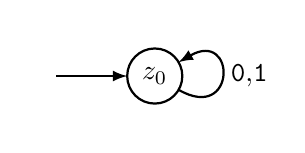
\begin{tikzpicture}[>=latex,thick]
\draw (0,0) circle[radius=0.35];
\node at (0,0) {$z_0$};
\draw[->,shorten <= 0.35cm,shorten >= 0.35cm] (-1.6,0) -- (0,0);
\draw[->,shorten <= 0.35cm,shorten >= 0.35cm]
	(0,0) to[out=-30,in=30,distance=1.2cm] (0,0);
\node at (1.2,0) {\texttt{0},\texttt{1}};
\end{tikzpicture}
\end{center}
Lösung mit Myhill-Nerode: Startzustand ist die Menge $L=\emptyset$
Da $\varepsilon\not\in\emptyset$ ist dieser Zustand kein Startzustand.
Ausserdem sind die $L(w)$ für jedes $w\in\Sigma_2^*$ weitere Zustände.
Nach Definition ist $L(w)=\{w_e\in\Sigma_2^*\,|\,ww_e\in \emptyset\}=\emptyset$,
es gibt also nur einen einzigen Zustand, damit ist der Automat bereits
vollständig definiert.
\qedhere
\end{teilaufgaben}
\end{loesung}

